\chapter{Poisson Brackets, Generators, and Angular Momentum}

We return in this lecture to Poisson brackets, but not as a separate ornament attached to Hamiltonian mechanics. The point, as Leonard Susskind keeps insisting, is that the same bracket that gives us time derivatives also packages rotations, translations, and the relation between symmetry and conservation. These notes follow that unfolding closely; this companion-note edition also carries credit to LazyingArt LLC and Video2Book. The route is deliberate: we begin with a recap, test the formalism on the harmonic oscillator, then turn to angular momentum, where Poisson brackets stop looking redundant and begin to show real power.

\section{From Hamilton's Equations to the Poisson Bracket}

The lecture opens by going back to a simple question. Suppose \(f(p,q)\) is any sufficiently smooth function on phase space. We may think of it as a quantity assigned to each point of phase space, but we may also think of it along a trajectory: as the system moves, the coordinates \(q_i\) and momenta \(p_i\) change, and therefore \(f\) changes too. What is its time derivative?

By the chain rule,
\begin{equation}
\dot f=\sum_i \frac{\partial f}{\partial q_i}\dot q_i+\sum_i \frac{\partial f}{\partial p_i}\dot p_i.
\end{equation}
Now substitute Hamilton's equations,
\begin{equation}
\dot q_i=\frac{\partial H}{\partial p_i},\qquad \dot p_i=-\frac{\partial H}{\partial q_i},
\end{equation}
and obtain
\begin{equation}
\dot f=\sum_i \frac{\partial f}{\partial q_i}\frac{\partial H}{\partial p_i}
-\sum_i \frac{\partial f}{\partial p_i}\frac{\partial H}{\partial q_i}.
\end{equation}

This combination occurs so often that it is natural to define it once and for all. For any two phase-space functions \(F\) and \(G\),
\begin{equation}
\{F,G\}=\sum_i \frac{\partial F}{\partial q_i}\frac{\partial G}{\partial p_i}
-\sum_i \frac{\partial F}{\partial p_i}\frac{\partial G}{\partial q_i}.
\end{equation}
With this notation,
\begin{equation}
\dot f=\{f,H\}.
\end{equation}

The important point is already visible. The bracket itself is defined for any pair \(F,G\). Only when the second entry is the Hamiltonian does it become a time derivative. The lecture will make repeated use of that distinction.

\section{The Algebra of Poisson Brackets and the Harmonic Oscillator}

Once the bracket has been isolated, Susskind pauses to treat it as a calculus. The rules are not arbitrary; they follow directly from the definition. The basic ones are
\begin{align}
\{A,B\}&=-\{B,A\},\\
\{A+B,C\}&=\{A,C\}+\{B,C\},\\
\{\lambda A,B\}&=\lambda\{A,B\},\\
\{AB,C\}&=A\{B,C\}+\{A,C\}B.
\end{align}
From antisymmetry we immediately have
\begin{equation}
\{A,A\}=0.
\end{equation}
And the canonical special cases are
\begin{equation}
\{q_i,q_j\}=0,\qquad \{p_i,p_j\}=0,\qquad \{q_i,p_j\}=\delta_{ij}.
\end{equation}

The lecture now insists on a concrete example. Let us use the bracket rules alone, together with the dynamical rule \(\dot A=\{A,H\}\), and recover the motion of the harmonic oscillator. Take
\begin{equation}
H=\frac{p^2}{2m}+\frac{k}{2}q^2.
\end{equation}
Then
\begin{align}
\dot q
&=\{q,H\}\\
&=\left\{q,\frac{p^2}{2m}+\frac{k}{2}q^2\right\}\\
&=\frac{1}{2m}\{q,p^2\},
\end{align}
because \(q\) has zero Poisson bracket with any function of \(q\). Using the Leibniz rule,
\begin{align}
\{q,p^2\}&=\{q,pp\}=p\{q,p\}+\{q,p\}p=2p,
\end{align}
and therefore
\begin{equation}
\dot q=\frac{p}{m}.
\end{equation}

Now do the same for \(p\):
\begin{align}
\dot p
&=\{p,H\}\\
&=\left\{p,\frac{p^2}{2m}+\frac{k}{2}q^2\right\}\\
&=\frac{k}{2}\{p,q^2\},
\end{align}
because \(p\) has zero Poisson bracket with any function of \(p\). Again,
\begin{align}
\{p,q^2\}&=\{p,qq\}=q\{p,q\}+\{p,q\}q=-2q,
\end{align}
so that
\begin{equation}
\dot p=-kq.
\end{equation}
Combining the two,
\begin{equation}
m\ddot q=-kq.
\end{equation}

The oscillator is the lecture's first full test case. It shows that Poisson brackets do reproduce the equations of motion. But Susskind immediately marks the limitation: so far the method has mostly repackaged Hamilton's equations. The next move is the essential one. The real power appears when we Poisson bracket with a conserved quantity other than the Hamiltonian.

\section{Angular Momentum From Rotational Symmetry}

The lecture now pivots. Angular momentum is recalled not as a memorized formula, but as the conserved quantity associated with rotational symmetry. For an infinitesimal symmetry of the form
\begin{equation}
\delta q_i=F_i(q)\,\epsilon,
\end{equation}
the conserved quantity is
\begin{equation}
Q=\sum_i p_i F_i(q).
\end{equation}
As in the lecture, we suppress the overall factor of \(\epsilon\), since multiplying a conserved quantity by a fixed constant changes nothing essential.

For a rotation about the \(z\)-axis,
\begin{equation}
\delta x=-y\,\epsilon,\qquad \delta y=x\,\epsilon,\qquad \delta z=0.
\end{equation}
Substituting these variations gives
\begin{equation}
L_z=p_x(-y)+p_yx=xp_y-yp_x.
\end{equation}
This is angular momentum in the plane, but it is more naturally read as the \(z\)-component of a three-dimensional vector.

Cycling the coordinates yields the other components:
\begin{equation}
L_x=yp_z-zp_y,\qquad
L_y=zp_x-xp_z,\qquad
L_z=xp_y-yp_x.
\end{equation}
Equivalently,
\begin{equation}
\mathbf L=\mathbf r\times\mathbf p.
\end{equation}
If we want the conserved quantity associated with rotation about an arbitrary axis \(\hat n\), we take
\begin{equation}
L_{\hat n}=\hat n\cdot \mathbf L.
\end{equation}

This finishes one part of the story. We have reconstructed angular momentum from symmetry. The lecture now asks the sharper question: once we have \(L_z\), what does Poisson bracketing with \(L_z\) actually do?

\section{Angular Momentum as Generator of Rotations}

Before bracketing angular momentum with itself, Susskind deliberately explores what happens when we bracket \(L_z\) with ordinary phase-space variables. The mood here is not theorem-proof-corollary. It is exploratory: let us see what the bracket knows.

Using
\[
L_z=xp_y-yp_x,
\]
we find
\begin{align}
\{x,L_z\}&=-y,\\
\{y,L_z\}&=x,\\
\{z,L_z\}&=0.
\end{align}
These are exactly the infinitesimal rotation formulas we started from. For instance, \(\{x,L_z\}\) gets a contribution only from the \(p_x\) term inside \(L_z\), and that contribution is \(-y\). Likewise \(\{y,L_z\}=x\), and \(z\) is unchanged.

The same pattern holds for momentum:
\begin{align}
\{p_x,L_z\}&=-p_y,\\
\{p_y,L_z\}&=p_x,\\
\{p_z,L_z\}&=0.
\end{align}
This is not an accident. Momentum is a vector, and the bracket with \(L_z\) rotates its components in the same way that it rotates the position vector.

\subsection{Question \& Answer}

\paragraph{Question.} What does Poisson bracketing with angular momentum actually do?

\paragraph{Answer.} It gives the infinitesimal change of a quantity under rotation. In the present case,
\begin{equation}
\delta A=\epsilon\,\{A,L_z\}
\end{equation}
is the infinitesimal transformation of any phase-space function \(A\) under a small rotation about the \(z\)-axis. Thus
\[
\delta x=-y\,\epsilon,\qquad \delta y=x\,\epsilon,\qquad \delta z=0,
\]
and similarly for the momentum components.

At this level, the lecture treats this almost as a definition in Hamiltonian language: given a quantity \(G\), we can associate to it an infinitesimal transformation by Poisson bracketing with \(G\). Whether that transformation is a symmetry is a separate question, one that will be tied to conservation shortly. But the transformation itself is already sitting in the bracket.

This is the first place where the analogy with the Hamiltonian becomes fully visible. The Hamiltonian generates small shifts in time through
\[
\dot A=\{A,H\}.
\]
Angular momentum generates small rotations through the same structure.

\section{Momentum, Translation, and the General Generator Idea}

Once the rotational case is understood, the lecture immediately tries another one. If momentum is the conserved quantity associated with translation invariance, does Poisson bracketing with momentum generate translation in the same way that Poisson bracketing with angular momentum generated rotation?

For a one-dimensional translation,
\begin{equation}
\delta q=\epsilon.
\end{equation}
In the symmetry formula \(\delta q=F(q)\epsilon\), this corresponds to \(F=1\), so the conserved quantity is simply
\begin{equation}
Q=p.
\end{equation}
The suggestion now hanging in the air is clear: for a function \(f(q)\), does \(\{f(q),p\}\) give \(df/dq\), the small change of \(f\) under a shift of \(q\)?

\subsection{Question \& Answer}

\paragraph{Question.} Does Poisson bracketing with momentum really give the infinitesimal translation?

\paragraph{Answer.} Yes. The lecture proves it first for powers of \(q\), by induction, because that is the cleanest place to see the mechanism.

\begin{proof}
For \(n=1\),
\[
\{q,p\}=1,
\]
so the statement holds.

Assume now that
\[
\{q^{n-1},p\}=(n-1)q^{n-2}.
\]
Then
\begin{align}
\{q^n,p\}
&=\{q\,q^{n-1},p\}\\
&=q\{q^{n-1},p\}+\{q,p\}q^{n-1}\\
&=q\bigl((n-1)q^{n-2}\bigr)+q^{n-1}\\
&=nq^{n-1}.
\end{align}
Thus, if the claim holds for \(n-1\), it holds for \(n\), and since it holds for \(n=1\), it holds for all positive integers \(n\).
\end{proof}

Therefore
\begin{equation}
\{q^n,p\}=nq^{n-1}.
\end{equation}
By linearity, constant extraction, and the usual extension from polynomials to smooth functions, we obtain the local general rule
\begin{equation}
\{f(q),p\}=\frac{df}{dq}.
\end{equation}

This is the second nontrivial example, and it seals the pattern. Momentum generates translations. Angular momentum generates rotations. The Hamiltonian generates time translations. Susskind jokes that we need a verb and proposes ``Poissonate.'' The joke is only in the name. The idea itself is exact: Poisson bracketing with the appropriate generator gives the infinitesimal change under the associated transformation.

\section{Conservation and Symmetry in One Equation}

Having built the generator idea from examples, the lecture now turns to the relation between generators, symmetries, and conserved quantities. Let \(G(q,p)\) be any phase-space function. In Hamiltonian language, we may associate to it the infinitesimal transformation
\begin{equation}
\delta_G A=\epsilon\,\{A,G\}.
\end{equation}
By itself this does not yet say that the transformation is a symmetry. It simply says that every phase-space function \(G\) defines an infinitesimal transformation rule.

Now add the extra condition that \(G\) is conserved. Since time evolution is generated by \(H\), that condition is
\begin{equation}
\dot G=\{G,H\}=0.
\end{equation}
Using antisymmetry, we may write the same statement as
\begin{equation}
\{H,G\}=0.
\end{equation}
The content of the lecture lies in reading these two lines differently. The first says that \(G\) does not change in time. The second says that the Hamiltonian does not change under the transformation generated by \(G\). One and the same vanishing bracket therefore says two things at once: conservation of \(G\), and symmetry of \(H\).

\begin{figure}[h]
\centering

\includegraphics[width=0.66\textwidth]{lecture_08_figure_02.png}
\caption{The lecture isolates the two orders of the same vanishing Poisson bracket so that the two readings are impossible to miss: \(G\) is conserved, and \(H\) is invariant under the transformation generated by \(G\).}
\end{figure}

This is why the board frame matters. The lecture does not bury the two equations in a derivation. It writes them one above the other, with almost nothing else on the board:
\begin{align}
\{G,H\}&=0,\\
\{H,G\}&=0.
\end{align}

\subsection{Question \& Answer}

\paragraph{Question.} If we know what is conserved, can we recover the symmetry?

\paragraph{Answer.} Yes. If a quantity \(G\) is conserved, then we bracket everything in sight with \(G\), and those brackets tell us how the variables transform:
\[
\delta_G A=\epsilon\,\{A,G\}.
\]
That is precisely what the lecture says. If we did not already know that angular momentum corresponds to rotation, the brackets with \(L_z\) would tell us. If we did not already know that momentum corresponds to translation, the brackets with \(p\) would tell us.

But there is an important clarification, and the lecture spends time on it. These are not, by themselves, equations of motion. They become equations of motion only when the distinguished quantity inside the bracket is the Hamiltonian. Otherwise they describe symmetry transformations, not the actual time development of the system.

This is where the chapter must not become too textbook-like. The live discussion matters. The student question is exactly the right one: does a conserved quantity tell us how things move? The answer is no, not directly. It tells us what symmetry operation is associated with the conservation law. Dynamics still comes from \(H\).

\section{Angular-Momentum Algebra and the Gyroscope}

Now that we have seen angular momentum acting on coordinates and momenta, the lecture returns to angular momentum itself. The next step is to compute the Poisson brackets of one component of \(\mathbf L\) with another and to use that algebra as a stand-alone dynamical structure.

Let us compute one example explicitly:
\begin{align}
\{L_x,L_z\}
&=\{yp_z-zp_y,\;xp_y-yp_x\}\\
&=\{yp_z,\;xp_y\}+\{-zp_y,\;-yp_x\}\\
&=xp_z-zp_x\\
&=-(zp_x-xp_z)\\
&=-L_y.
\end{align}
The lecture then reverses the order to remove the minus sign and cycles the coordinates. In the familiar cyclic form we have
\begin{equation}
\{L_x,L_y\}=L_z,\qquad
\{L_y,L_z\}=L_x,\qquad
\{L_z,L_x\}=L_y.
\end{equation}

This is already the algebra we want. It is the classical Poisson-bracket precursor of the angular-momentum commutation relations of quantum mechanics, though the lecture deliberately does not go further into that story here. More importantly for the present course, it means we can solve problems using the \(L_i\) directly, without dragging ourselves back through the underlying particle coordinates each time.

\subsection{The Gyroscope}

The payoff example is the gyroscope. We imagine a rapidly spinning flywheel whose center remains at a fixed distance from a pivot. The lecture is careful, if somewhat notationally unstable, about what this means. The slanted direction drawn on the board is best understood not as a mysterious axis with many names, but as the position vector \(\mathbf r\) from the pivot to the center of the wheel. The crucial approximation is that the dominant angular momentum stays aligned with that direction.

In a clean reconstruction, we write
\begin{equation}
\mathbf L=\ell\,\mathbf r,
\end{equation}
where \(\ell\) is approximately constant because the spin is assumed very large. In particular,
\begin{equation}
L_z=\ell z.
\end{equation}
This is not an exact identity for a general rigid body. It is the lecture's fast-gyroscope approximation. The later student questions make clear why the fixed-length assumption matters: without it, the proportionality between height and \(L_z\) would fail.

\begin{figure}[h]
\centering

\includegraphics[width=0.60\textwidth]{lecture_08_figure_03.png}
\caption{The first clear appearance of the gyroscope geometry on the board: vertical \(z\)-axis, pivot, slanted position direction, and the tilted flywheel.}
\end{figure}

\begin{figure}[h]
\centering
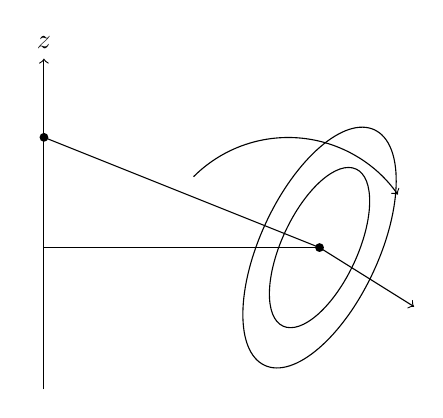
\begin{tikzpicture}[scale=1.0]
\draw[->] (0,0) -- (0,4.2) node[above] {$z$};
\fill (0,3.2) circle (1.6pt);
\coordinate (C) at (3.5,1.8);
\draw (0,3.2) -- (C);
\fill (C) circle (1.6pt);
\draw (0,3.2) -- (0,1.8);
\draw (0,1.8) -- (C);
\begin{scope}[shift={(C)}, rotate=-25]
\draw (0,0) ellipse (0.75 and 1.65);
\draw (0,0) ellipse (0.48 and 1.10);
\end{scope}
\draw[->] (1.9,2.7) arc[start angle=135,end angle=35,radius=1.7];
\draw[->] (C) -- +(1.2,-0.75);
\end{tikzpicture}
\caption{A cleaned redraw of the geometric picture. The point on the vertical axis is the pivot, the slanted line is the position direction \(\mathbf r\), and the fast-spin approximation keeps \(\mathbf L\) aligned with that direction.}
\end{figure}

The first contribution to the Hamiltonian is the rotational energy,
\begin{equation}
H_{\mathrm{rot}}=\frac{1}{2I}\left(L_x^2+L_y^2+L_z^2\right),
\end{equation}
with the corrected coefficient \(1/(2I)\). Susskind briefly says the wrong coefficient and then fixes it on the fly; the corrected form is the one we keep.

Before adding gravity, the lecture asks us to ignore it altogether. No torque, no potential, just a spinning gyroscope in free space. Then
\begin{align}
\dot L_x
&=\{L_x,H_{\mathrm{rot}}\}\\
&=\frac{1}{2I}\Bigl(\{L_x,L_x^2\}+\{L_x,L_y^2\}+\{L_x,L_z^2\}\Bigr)\\
&=\frac{1}{2I}\Bigl(0+2L_y\{L_x,L_y\}+2L_z\{L_x,L_z\}\Bigr)\\
&=\frac{1}{I}\bigl(L_yL_z-L_zL_y\bigr)=0.
\end{align}
The same reasoning gives
\begin{equation}
\dot L_y=0,\qquad \dot L_z=0.
\end{equation}
So in the torque-free case the angular momentum vector remains fixed, just as it should.

\subsection{Question \& Answer}

\paragraph{Question.} Why is the gravitational potential proportional to \(L_z\)?

\paragraph{Answer.} Because the gravitational potential is proportional to the height of the wheel center, and in the fast-spin approximation the height changes exactly as the \(z\)-component of \(\mathbf L\) changes. If we choose the vertical axis to be \(z\), and if \(z\) increases upward, then
\begin{equation}
V=Mg\,z.
\end{equation}
But since \(\mathbf L=\ell\,\mathbf r\), we also have \(L_z=\ell z\). Therefore
\begin{equation}
V=cL_z,\qquad c=\frac{Mg}{\ell}>0.
\end{equation}

The fixed-distance assumption is essential here. One of the students asks exactly the right question: what if the wheel center were free to move radially? Then the simple proportionality between height and \(L_z\) would fail. The lecture's argument is not a generic rigid-body theorem; it is a controlled approximation for a rapidly spinning gyroscope whose axle direction and position direction stay locked together.

\begin{remark}
The clean board frame reproduced below still shows an earlier sign,
\[
V=-cL_z,
\]
which the lecture later revisits and corrects after the choice of \(z\)-axis and height convention is clarified. In these notes we take \(z\) upward, so larger \(z\) means larger potential energy, and the cleaned formula is \(V=+cL_z\).
\end{remark}

\begin{figure}[h]
\centering

\includegraphics[width=0.72\textwidth]{lecture_08_figure_04.png}
\caption{The board view that combines the gyroscope geometry, the rotational-energy term, and an earlier-sign version of the potential. The screenshot is kept as evidence of the live board staging; the text adopts the corrected sign convention.}
\end{figure}

The full Hamiltonian is therefore
\begin{equation}
H=\frac{1}{2I}\left(L_x^2+L_y^2+L_z^2\right)+cL_z.
\end{equation}
Now the useful simplification from a few moments ago becomes decisive. The bracket of any \(L_i\) with \(L_x^2+L_y^2+L_z^2\) vanishes, so the only term that drives the dynamics is the linear \(cL_z\) term:
\begin{align}
\dot L_z&=\{L_z,H\}=c\{L_z,L_z\}=0,\\
\dot L_x&=\{L_x,H\}=c\{L_x,L_z\}=-cL_y,\\
\dot L_y&=\{L_y,H\}=c\{L_y,L_z\}=cL_x.
\end{align}
Thus the vertical component remains fixed, while the horizontal components rotate into one another. The tilt angle stays essentially fixed in the fast-spin approximation, and the vector \(\mathbf L\) precesses about the \(z\)-axis.

The lecture is candid at this point: Susskind says he is tired and may have lost a sign. The sign convention adopted here is consistent with the choice \(V=+cL_z\). The physical point is the more important one, and it is exactly the point he wants to leave us with. We have not solved for Euler angles. We have not developed the full rigid-body formalism. We have jumped directly to the angular-momentum components and written their equations of motion almost immediately.

This is also why the lecture ends by comparing the result to spin precession in a magnetic field. The source of the torque may be gravity, magnetism, or something else entirely; once the Hamiltonian contains a term linear in a component of angular momentum, the Poisson algebra forces the same precessional structure.

\section{Summary}

The lecture begins by returning to the time derivative of an arbitrary phase-space function and identifying the Poisson bracket as the combination that keeps reappearing. It then turns that combination into a working calculus, tests it on the harmonic oscillator, and pivots to angular momentum, where the formalism finally reveals its real point. Bracketing with \(L_z\) generates infinitesimal rotations, bracketing with \(p\) generates infinitesimal translations, and bracketing with \(H\) generates time evolution. The same vanishing bracket \(\{G,H\}=0\) can be read as conservation of \(G\) or invariance of \(H\) under the \(G\)-generated transformation, and the angular-momentum algebra then makes the gyroscope almost immediate. The lecture stops there on purpose. It does not become a full treatment of rigid-body dynamics. Its message is sharper: once the right Poisson-bracket structure is in hand, mechanics can often be done directly in the variables that matter.